\documentclass{article}
\usepackage{amsmath}
\usepackage{amssymb}
\usepackage{graphicx}
\usepackage{hyperref}
\usepackage[version=4]{mhchem}

\title{Example 10}
\date{}

\begin{document}
\maketitle

(2002 China Middle School Math Contest) In the diagram, \(A B=a\) cm is the diameter of circle \(O\). Circle \(O_{1}\) has the diameter of \(A O\) and is congruent to circle \(O_{2}\), and both are tangent to circle \(O\) and to each other. Circle \(O_{3}\) and circle \(O_{4}\) are congruent and are tangent to circle \(O\), to circle \(O_{1}\) and to circle \(O_{2}\). Find the area of quadrilateral \(O_{1} O_{2} O_{3} O_{4}\).\\
\centering
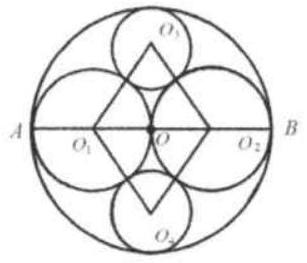
\includegraphics[width=\textwidth]{images/problem_image_1.jpg}

Solution: 1: 9.\\
Let the radius of the circle \(O\) be \(R\), the radius of the circle \(Q\) be \(r_{1}\), and the radius of the circle \(S\) be \(r_{2}\). We know that \(r_{1}=\frac{R}{2}\).\\
By the Pythagorean Theorem,\\
\(\left(R-r_{2}\right)^{2}=r_{1}^{2}+\left(r_{1}+r_{2}\right)^{2} \Rightarrow R^{2}-2 R r_{2}=2 r_{1} r_{2} \Rightarrow\)\\
\(R^{2}-2 R r_{2}=2 r_{1} r_{2} \Rightarrow r_{2}=\frac{R}{3}\).\\
\centering
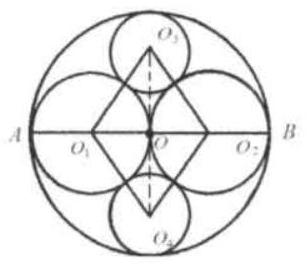
\includegraphics[width=\textwidth]{images/reasoning_image_1.jpg}

The ratio of the areas of the smallest circle and largest circle is \(\frac{\pi r_{2}{ }^{2}}{\pi R^{2}}=\frac{r_{2}{ }^{2}}{R^{2}}=\frac{\left(\frac{R}{3}\right)^{2}}{R^{2}}=\frac{1}{9}\).


\end{document}
